%!TEX root = ../talk.tex

\section{Numerical Comparisons}\label{sec:numer}

%%%

\frameinlbffalse

\begin{frame}[plain]
\frametitle{\S\ref{sec:numer}. \insertsection}
\listofframes
\end{frame}
\addtocounter{framenumber}{-1} % this page does not count

\frameinlbftrue


%%%
\subsection{Test setting}
%%%

\begin{frame}
	\MyLogo
	\frametitle{Hardware Platforms}  

\begin{itemize}

\item Use one quad-core desktop CPU (i.e., Intel i7-3820 CPU
		@ 3.60GHz) and two 8-core server-grade CPUs (i.e., Intel
		Xeon CPU E5-2630 v3 @ 2.40GHz)
		
\item Use two generations of GPU cards, GTX 1080 @ 1607MHz with
		Pascal architecture, and Telsa K80 @ 562MHz with Kepler
		architecture 
	\end{itemize}
	
\begin{figure}[htbp] 
	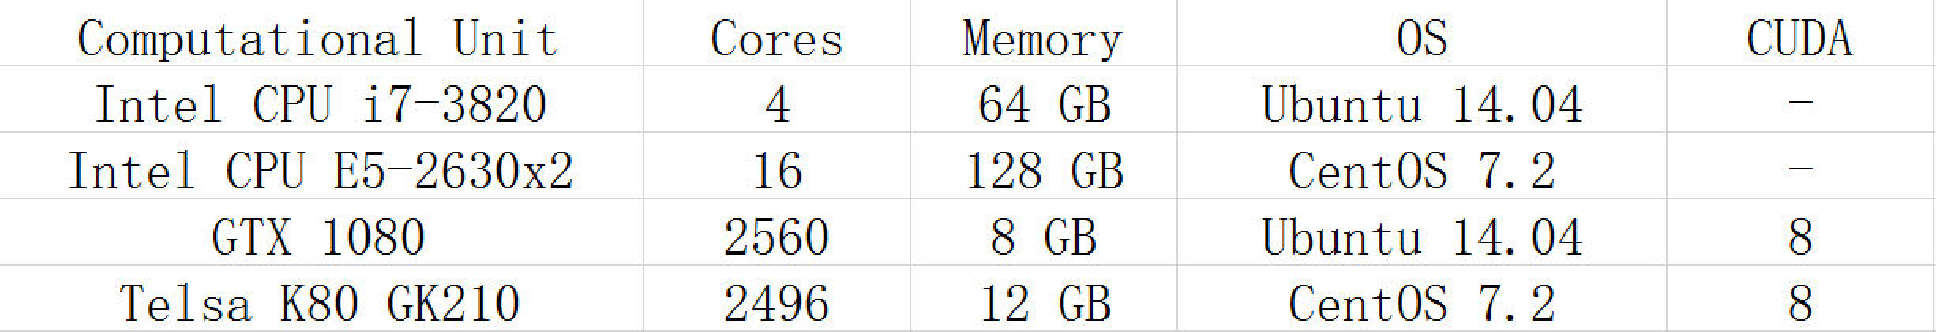
\includegraphics[height=1.2in]{figures/platforms.pdf} 
	\caption{The experimental hardware setting for data parallelization}
\end{figure}
	
\begin{center}
	{\color{red} \scriptsize
		Benchmarking State-of-the-Art Deep Learning Software Tools, by Shaohuai Shi, Qiang Wang.}
\end{center}

\end{frame}

%%%

\begin{frame}
  \MyLogo
  \frametitle{Neural Networks and Data Sets}  

\medskip

\begin{itemize}

\item A large fully-connected neural network (\alert{FCN-S}) with around 55 million parameters is used to evaluate the performance of FCN

\item The classical AlexNet (\alert{AlexNet-S}) is used as an representative of CNN

\item A smaller FCN (\alert{FCN-R}) is constructed for MNIST data set

\item An AlexNet (\alert{AlexNet-R}) architecture is used for Cifar10 data set

\item For RNNs, considering that the main computation complexity is related to the length of input sequence, 2 LSTM layers are selected for testing, with input length of 32.

\end{itemize}

\begin{figure}[htbp] 
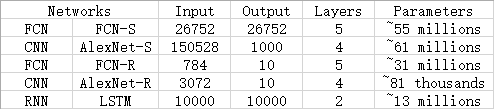
\includegraphics[height=1in]{figures/models.png} 
\caption{The experimental setup of neural networks for synthetic data and real data}
\end{figure}
	
\end{frame}

%%%
\subsection{CPU tests}
%%%

\begin{frame}
	\MyLogo
	\frametitle{CPU Scalability: FCN Synthetic}  
	\begin{figure}[htbp] 
		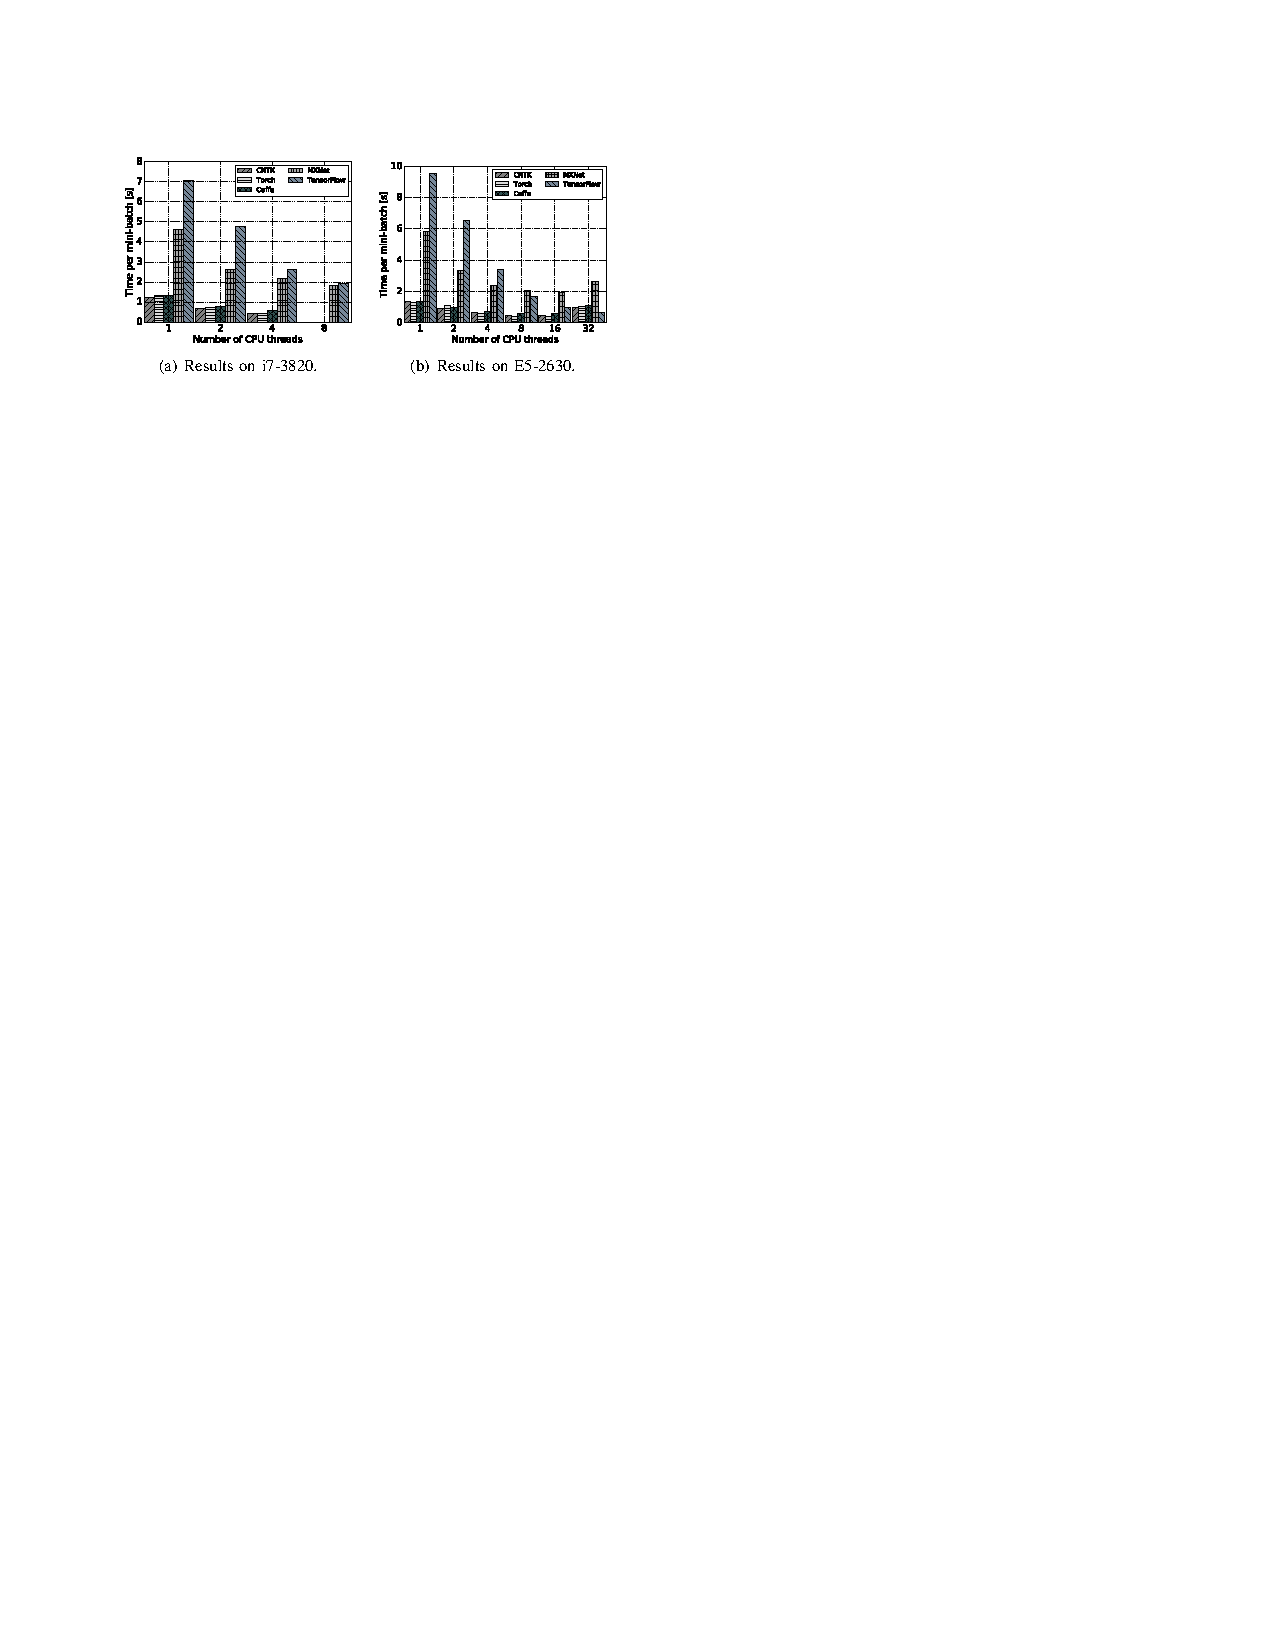
\includegraphics[height=2.2in]{figures/FCN-S1.pdf} 
		\caption{FCN-S performence comparison on CPU platform with a mini-batch size of 64.(The lower the better.)}
	\end{figure}
\end{frame}

%%%

\begin{frame}
	\MyLogo
	\frametitle{CPU Scalability: FCN Real}  
	\begin{figure}[htbp] 
		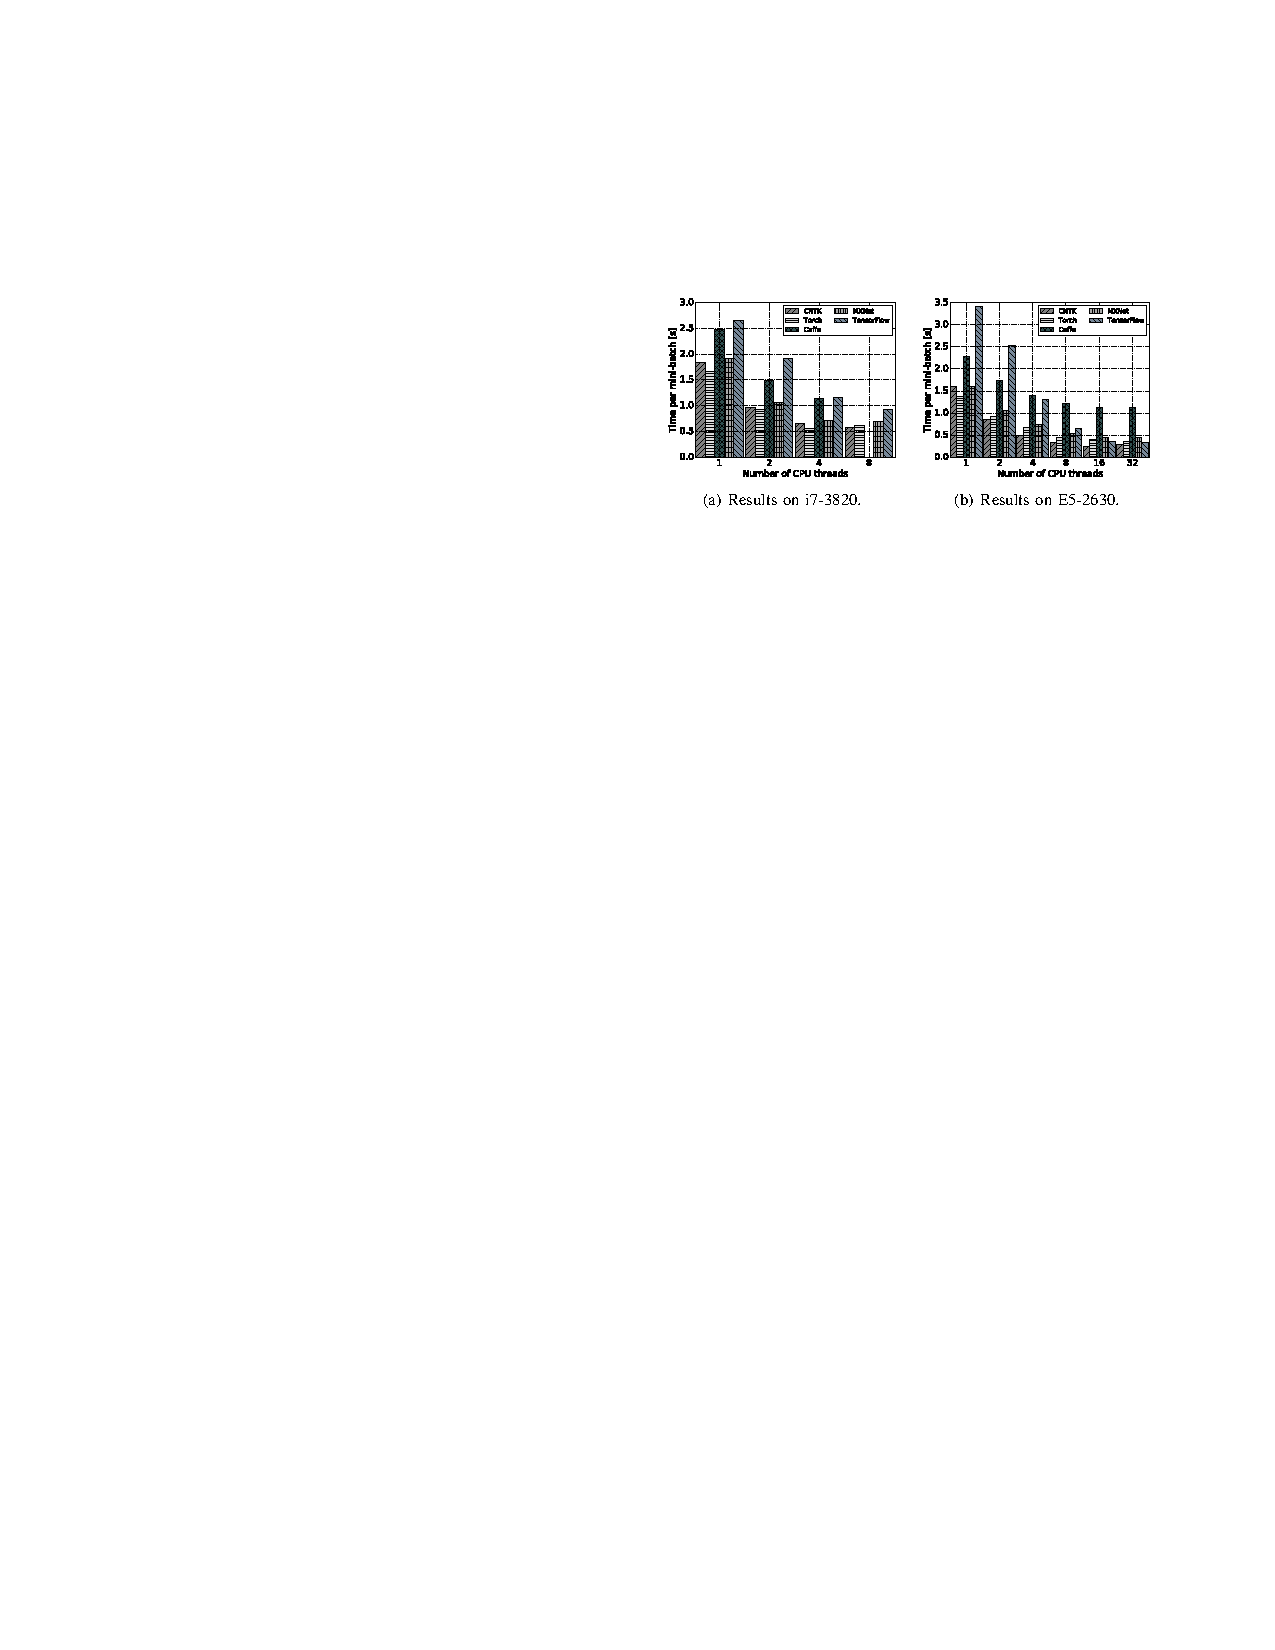
\includegraphics[height=2.2in]{figures/FCN-R1.pdf} 
		\caption{The FCN-R performance comparison on CPU platform with a mini-batch size of 1024.(The lower the better.)}
	\end{figure}
\end{frame}

%%%

\begin{frame}
	\MyLogo
	\frametitle{CPU Scalability: CNN Synthetic}  

	\begin{figure}[htbp] 
		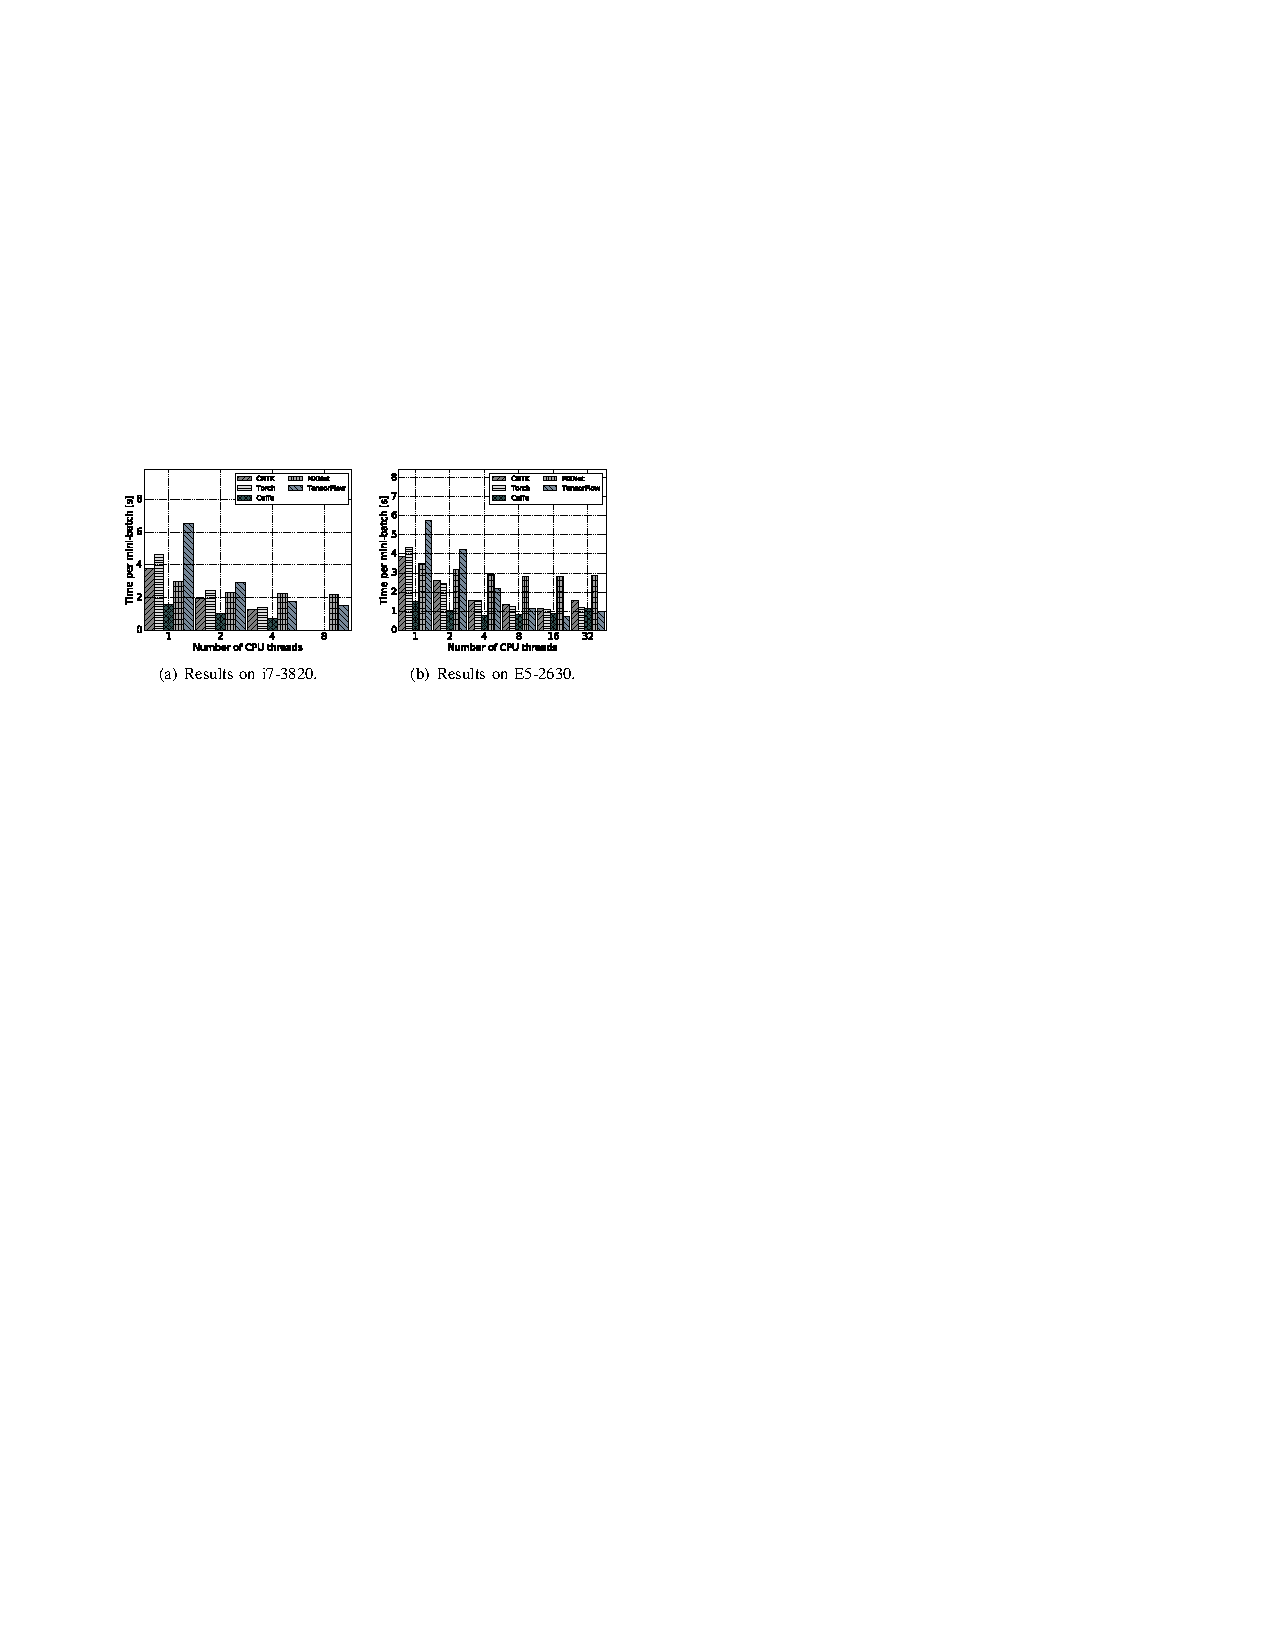
\includegraphics[height=2.2in]{figures/AlexNet-S1.pdf} 
		\caption{AlexNet-S performance comparison on CPU platform with a mini-batch size of 16 (The lower the better.)}
	\end{figure}	
\end{frame}

%%%

\begin{frame}
	\MyLogo
	\frametitle{CPU Scalability: CNN Real}  
	\begin{figure}[htbp] 
		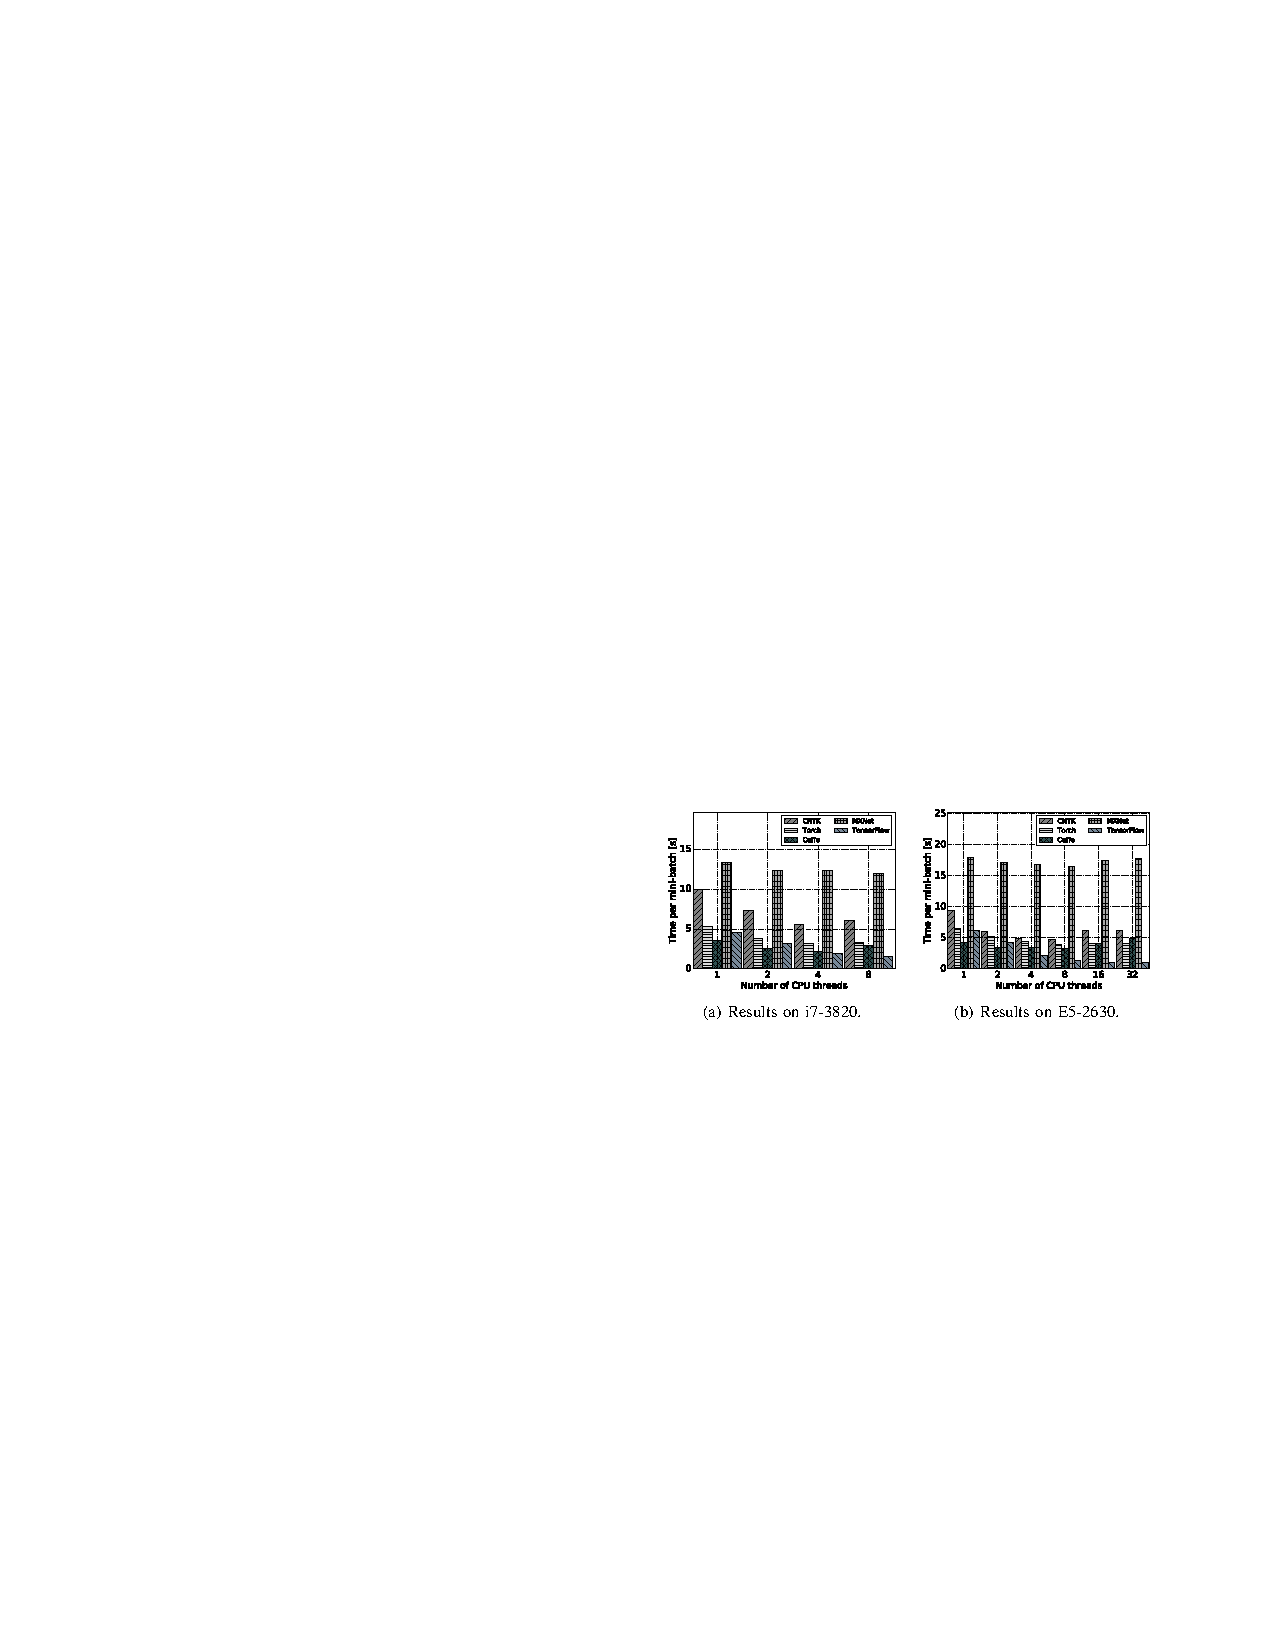
\includegraphics[height=2.2in]{figures/AlexNet-R1.pdf} 
		\caption{AlexNet-R performance comparison on CPU platform with a mini-batch size of 1024.(The lower the better.)}
	\end{figure}
\end{frame}

%%%

\begin{frame}
	\MyLogo
	\frametitle{CPU Scalability: RNN}  
	\begin{figure}[htbp] 
		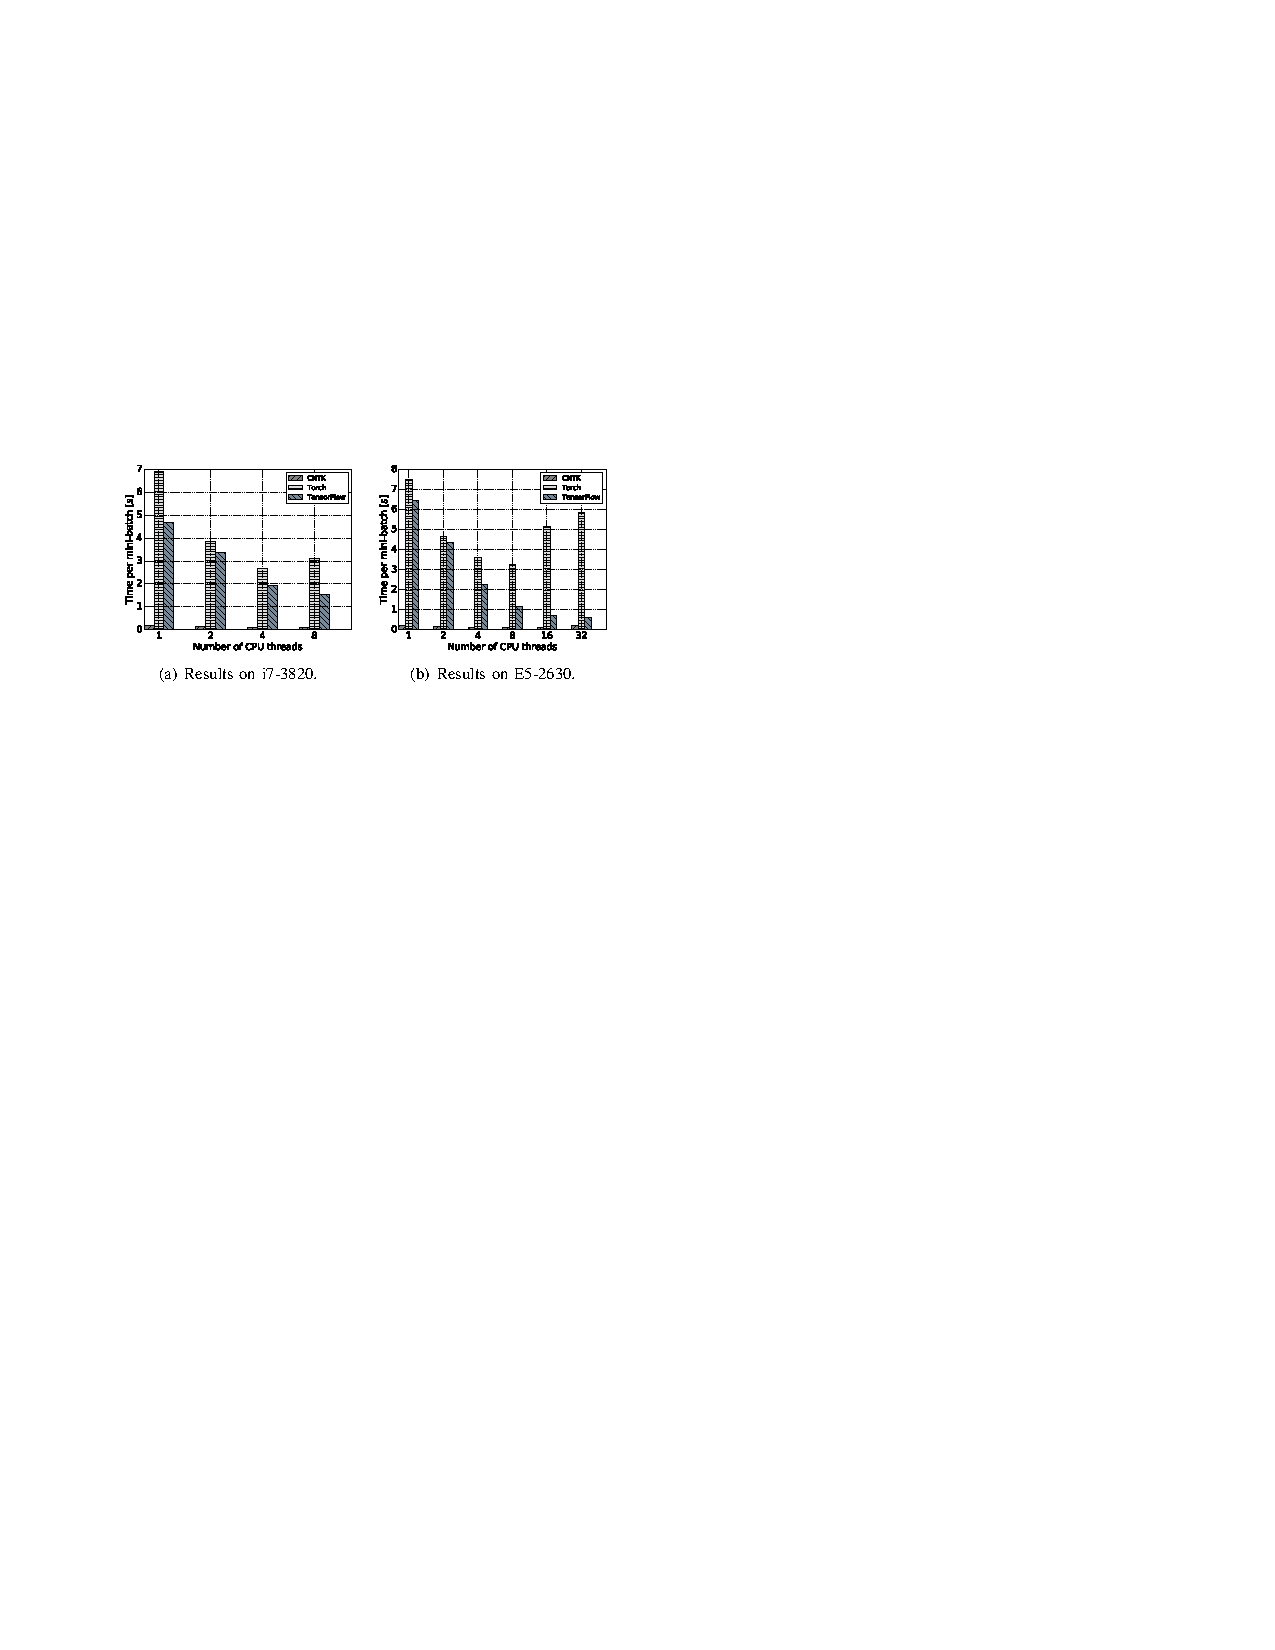
\includegraphics[height=2.2in]{figures/LSTM1.pdf} 
		\caption{LSTM performance comparison on CPU platform with a mini-batch size of 256.(The lower the better.)}
	\end{figure}
\end{frame}

%%%
\subsection{GPU tests}
%%%

\begin{frame}
	\MyLogo
	\frametitle{GPU Scalability: FCN Synthetic}

	\begin{figure}[htbp] 
		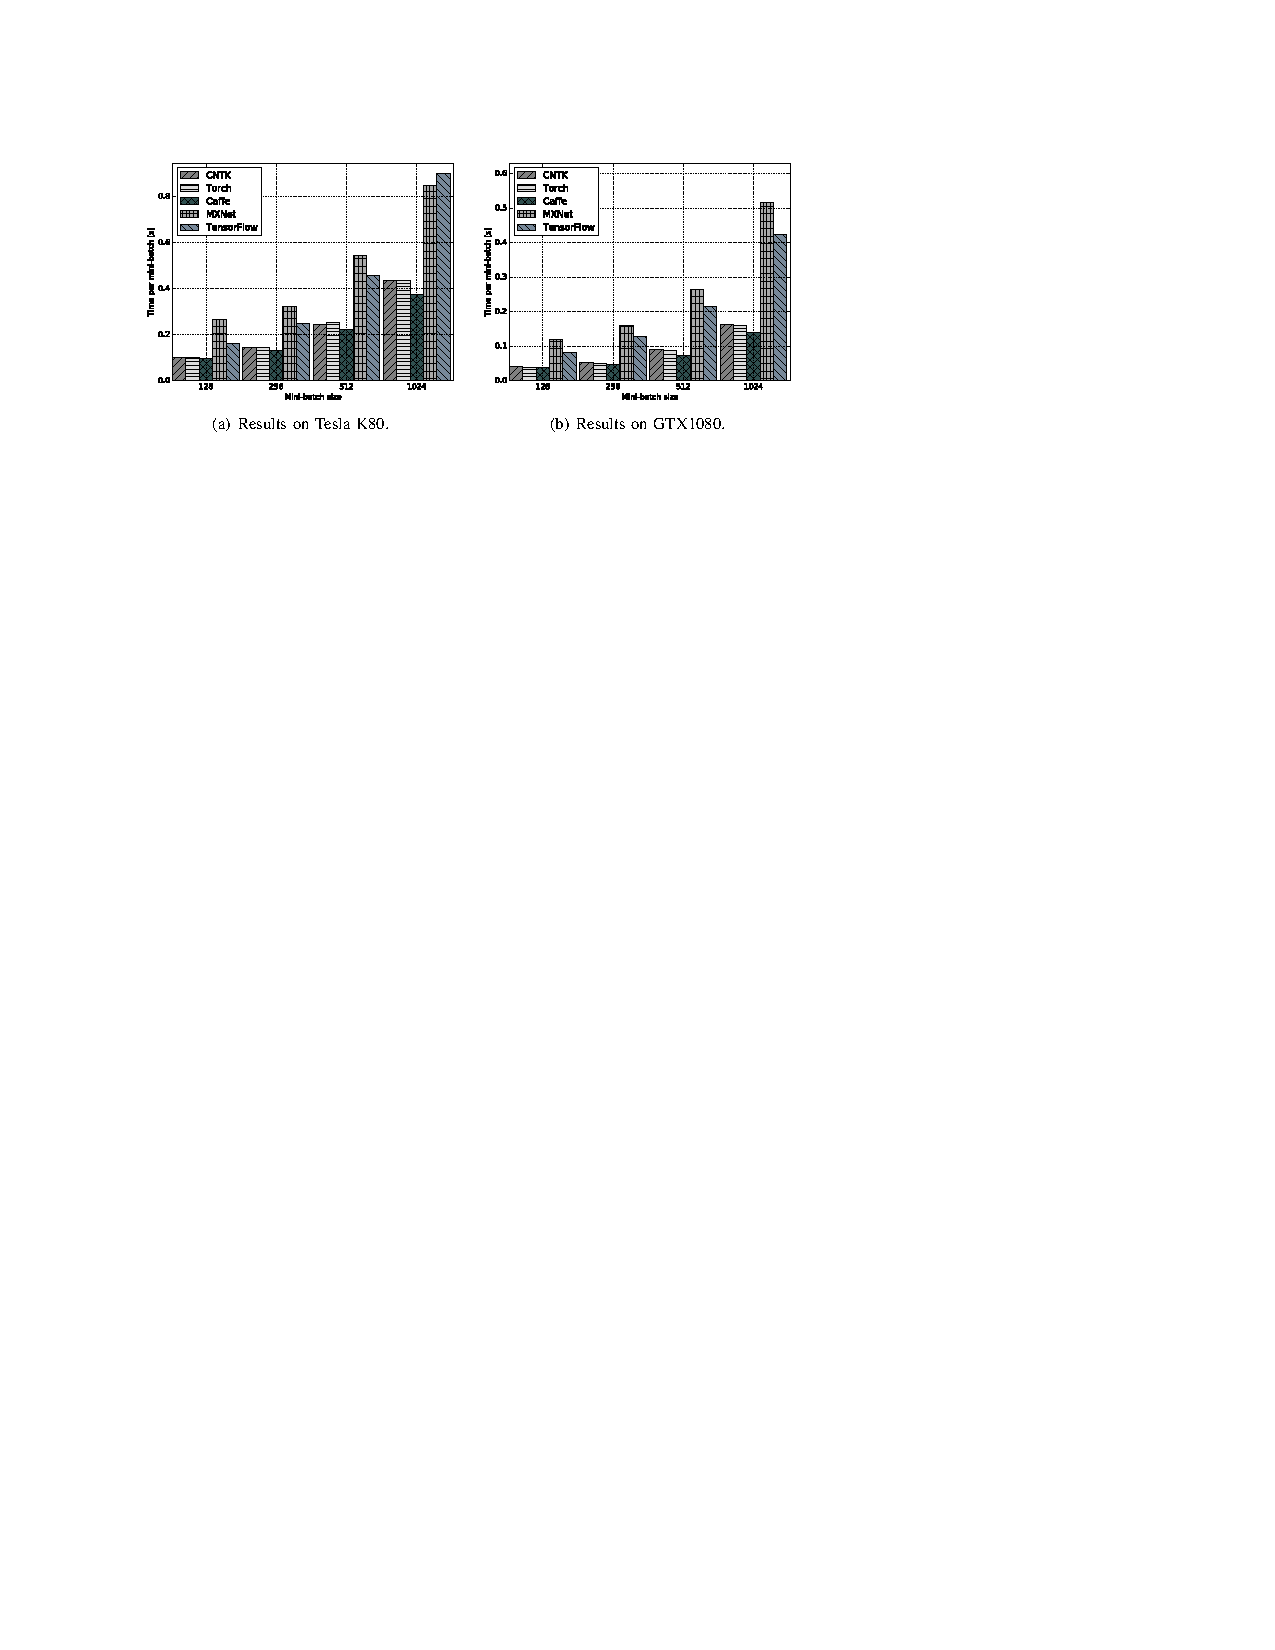
\includegraphics[height=1.8in]{figures/FCN-S2.pdf} 
		\caption{The performance comparison of FCN-S on GPU platforms.}
	\end{figure}

\end{frame}

%%%

\begin{frame}
	\MyLogo
	\frametitle{GPU Scalability: CNN Synthetic}

	\begin{figure}[htbp] 
		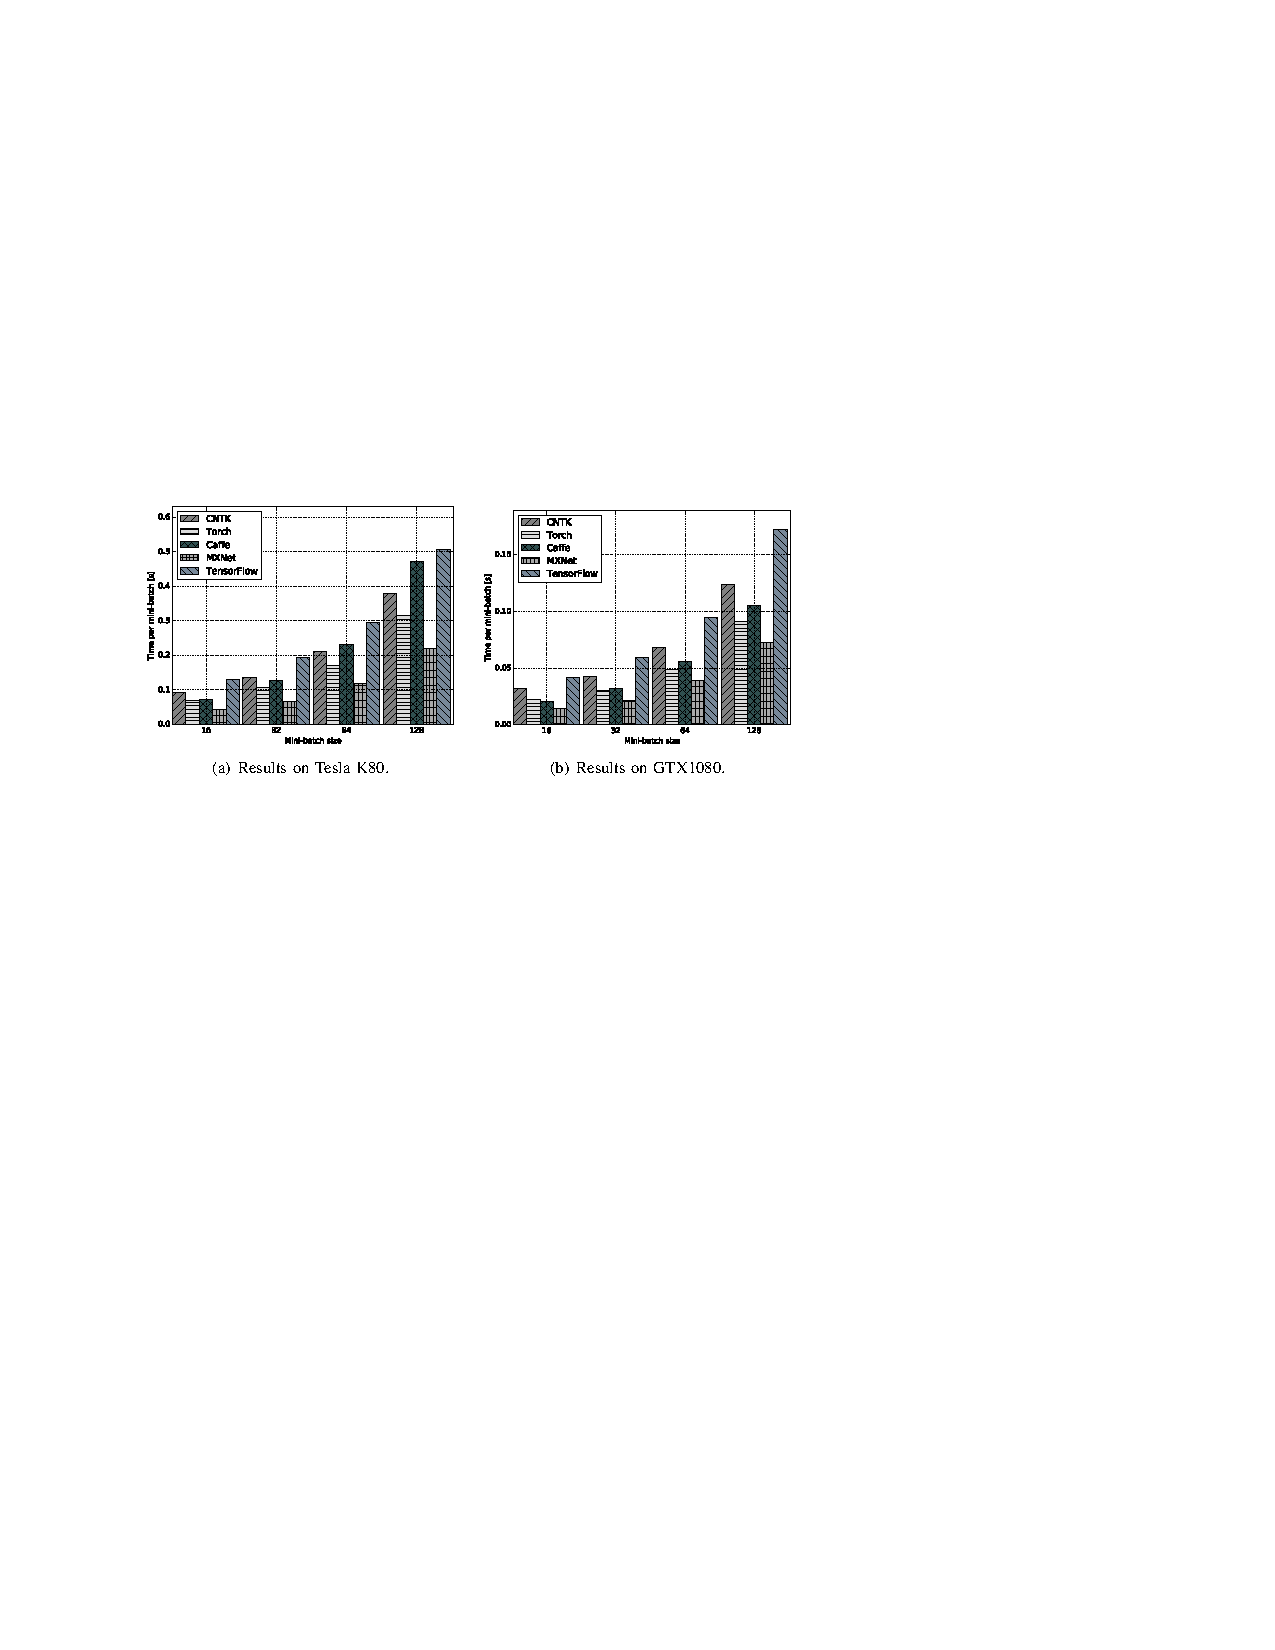
\includegraphics[height=1.8in]{figures/AlexNet-S2.pdf} 
		\caption{The performance comparison of AlexNet-S on GPU platforms.}
	\end{figure}

\end{frame}

%%%

\begin{frame}
	\MyLogo
	\frametitle{GPU Scalability: CNN Real}

	\begin{figure}[htbp] 
		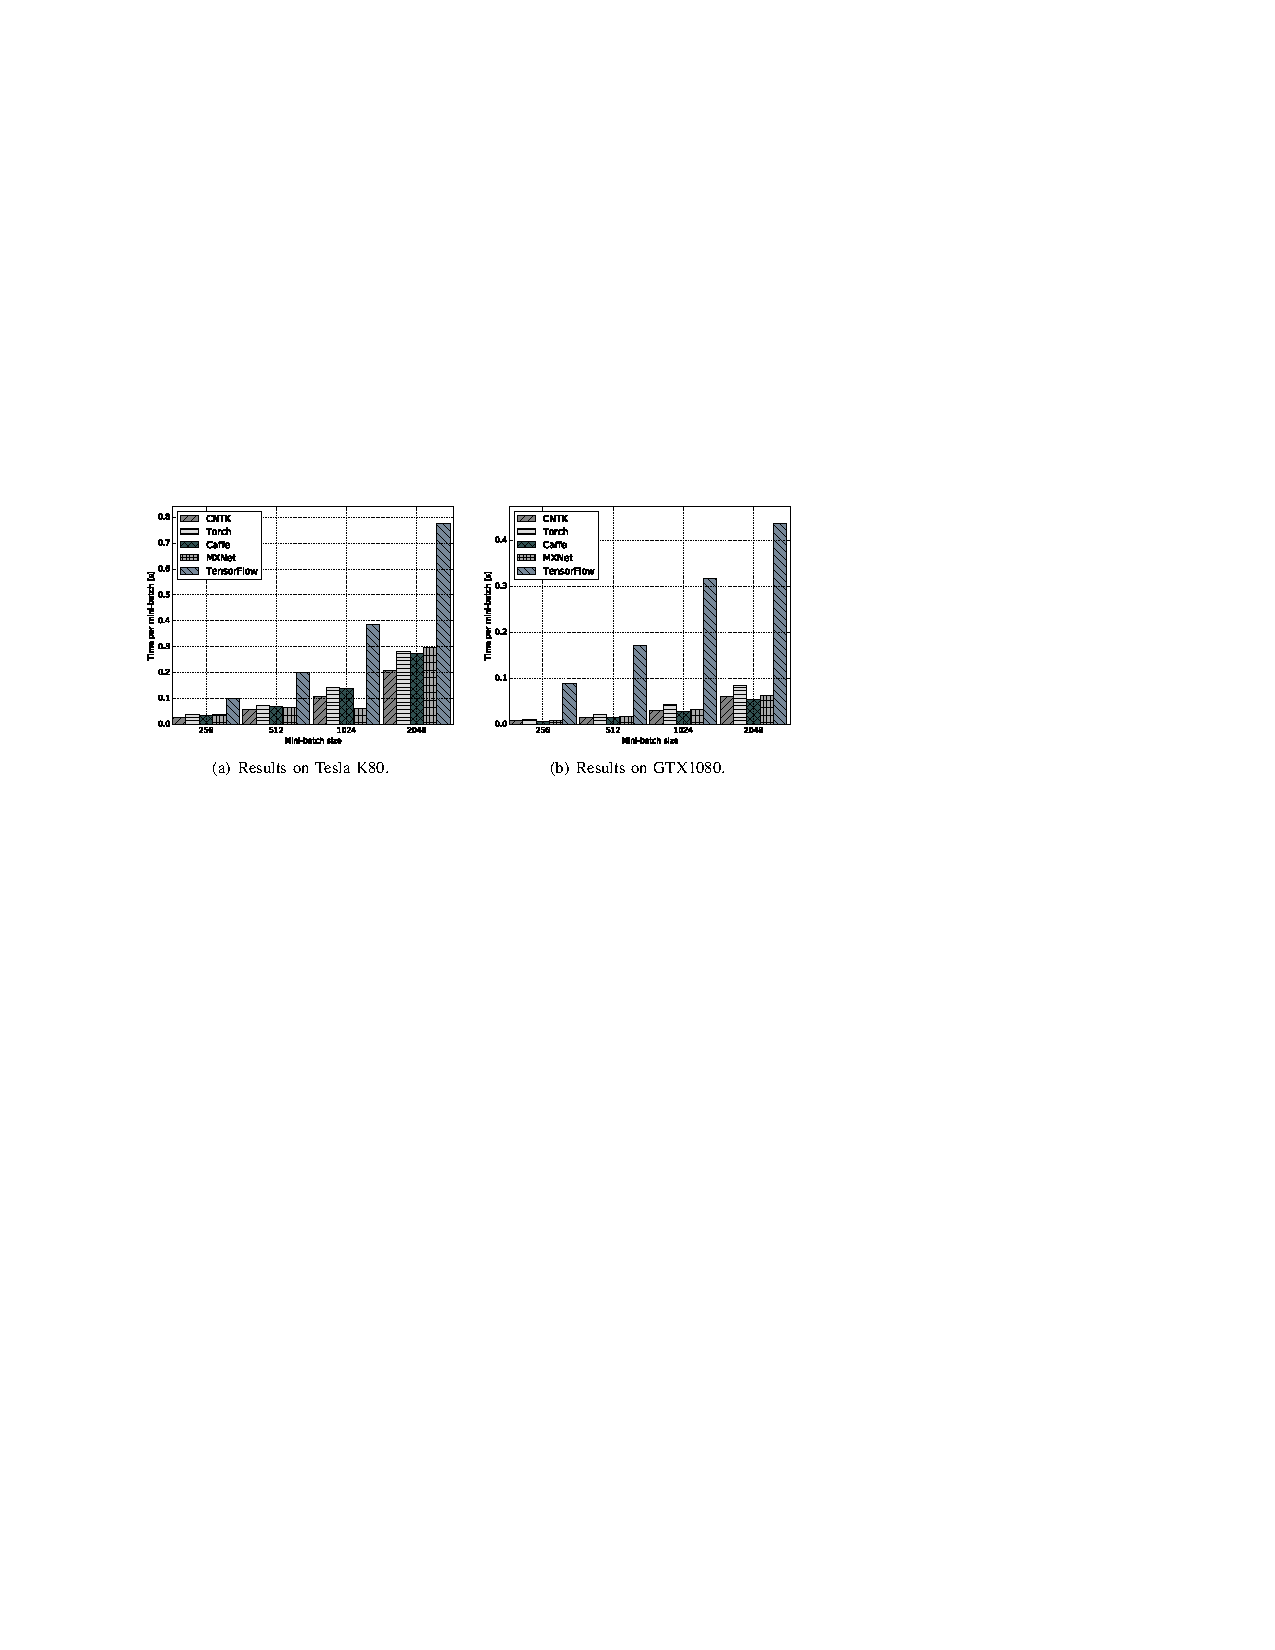
\includegraphics[height=1.8in]{figures/AlexNet-R2.pdf} 
		\caption{The performance comparison of AlexNet-R on GPU platforms.}
	\end{figure}

\end{frame}

%%%

\begin{frame}
	\MyLogo
	\frametitle{GPU Scalability: RNN Real}
	
	\begin{figure}[htbp] 
		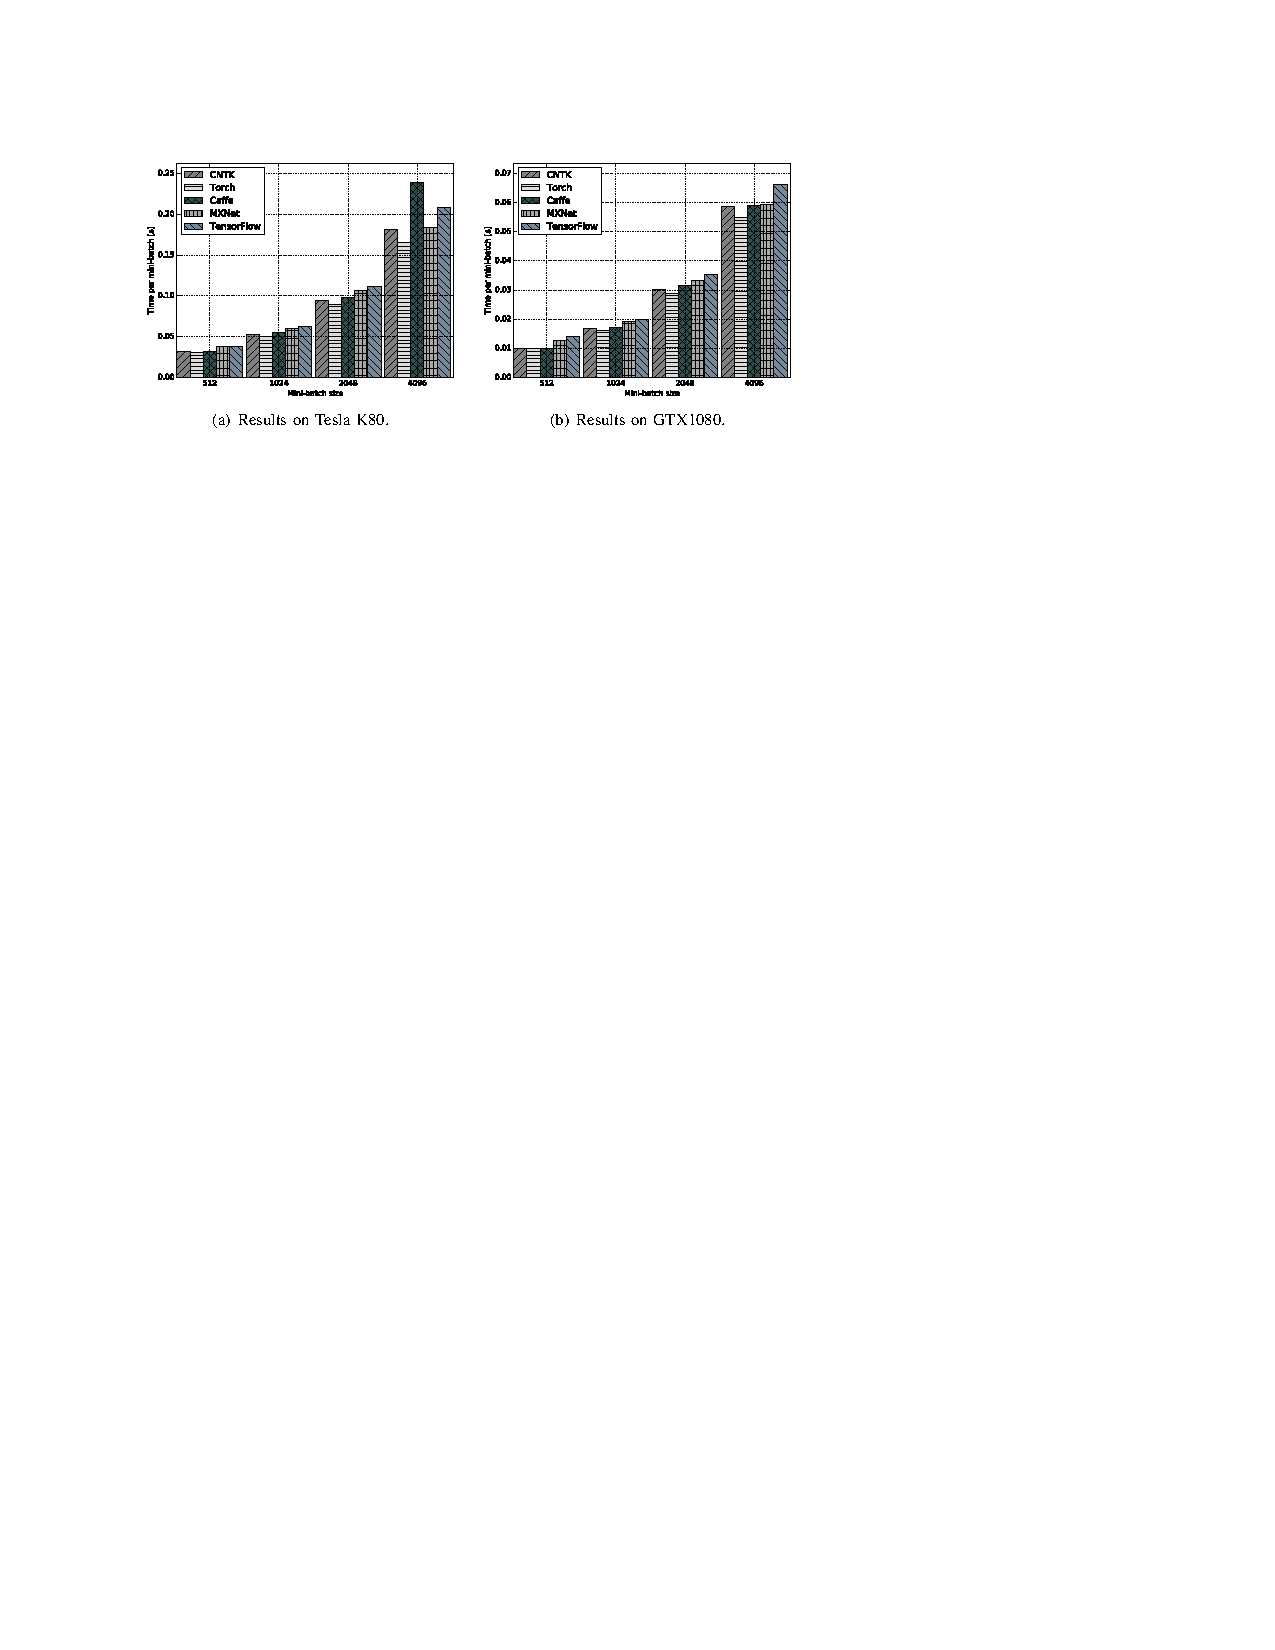
\includegraphics[height=1.8in]{figures/FCN-R2.pdf} 
		\caption{The performance comparison of FCN-R on GPU platforms.}
	\end{figure}

\end{frame}

%%%

\begin{frame}
	\MyLogo
	\frametitle{GPU Scalability: LSTM}
	
	\begin{figure}[htbp] 
		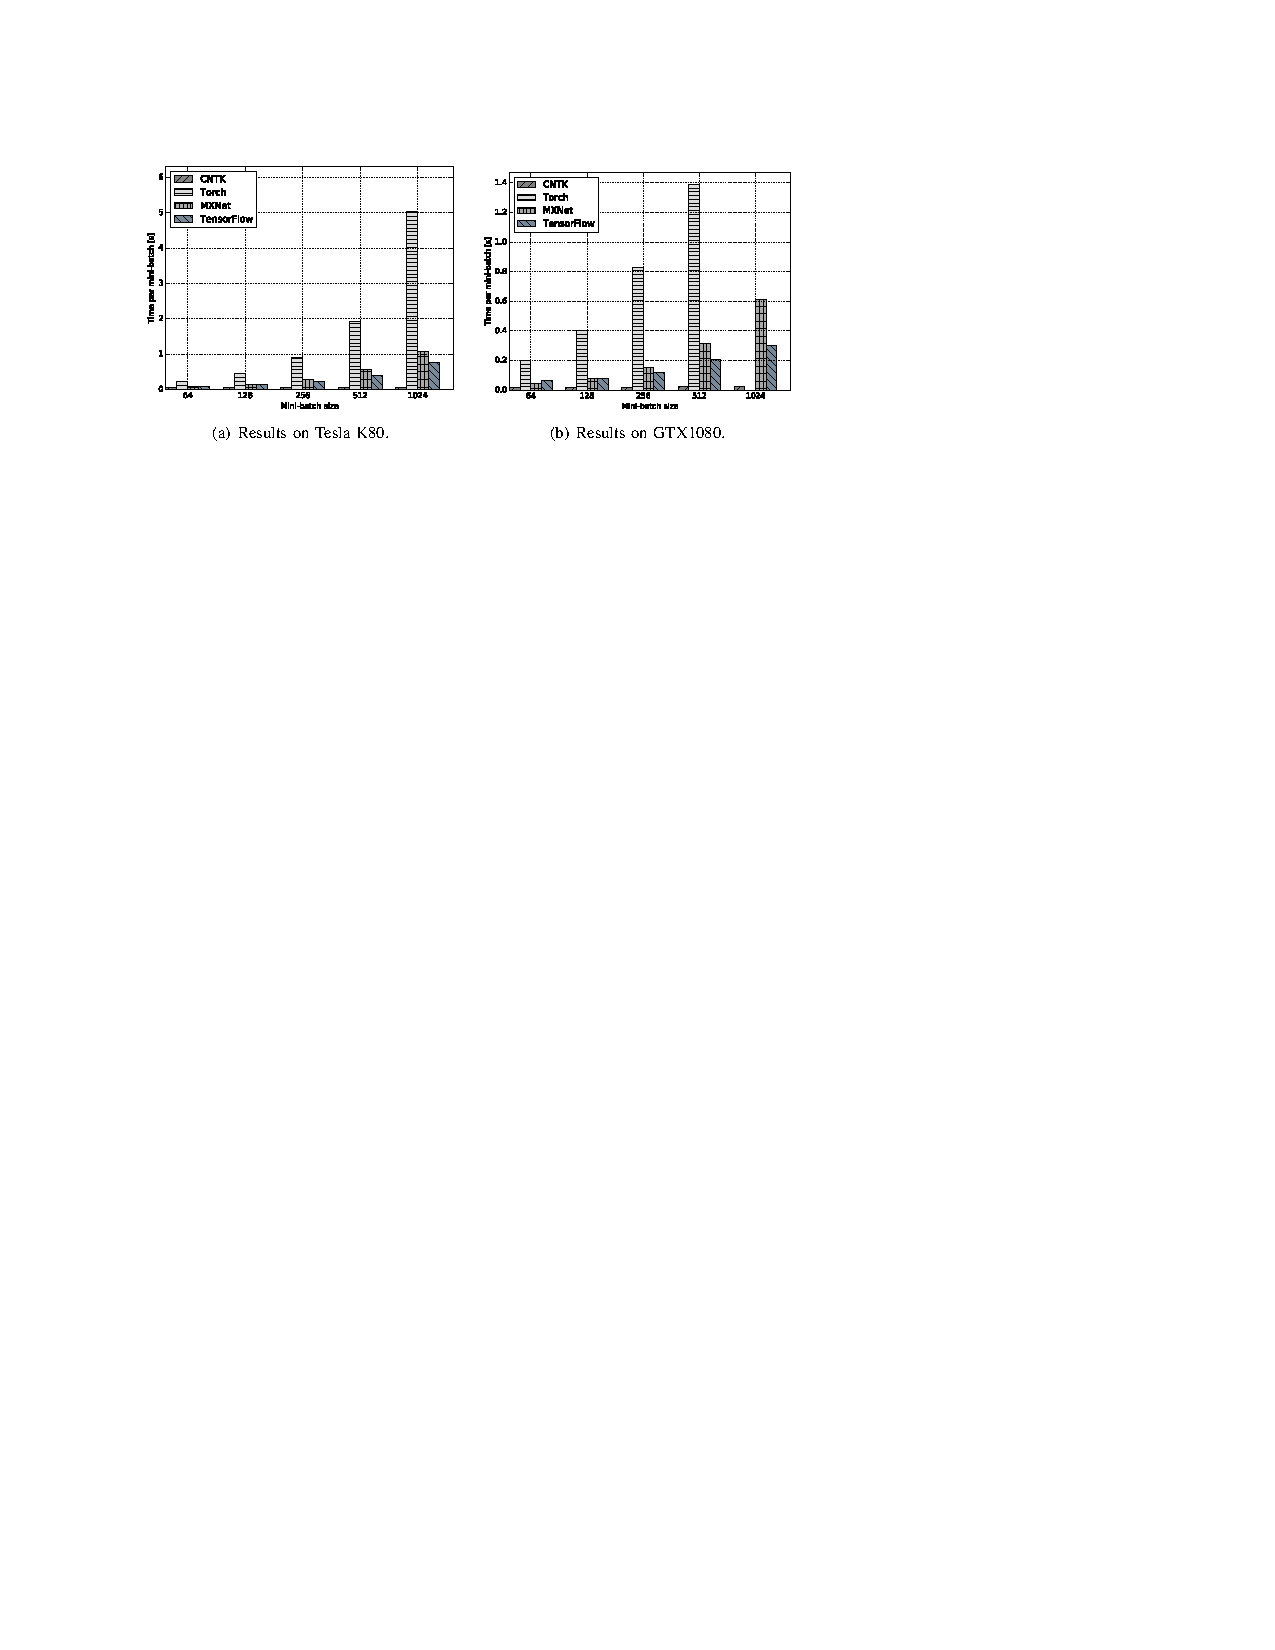
\includegraphics[height=2.0in]{figures/LSTM2.pdf} 
		\caption{The performance comparison of LSTM on GPU platforms.}
	\end{figure}
	
\end{frame}